\documentclass[12]{amsart}

\usepackage{amsmath}
\usepackage{amsthm}
\usepackage{tikz}
\usepackage{tikz-3dplot}
\usepackage{minted}
\usetikzlibrary{calc,patterns,angles,quotes,positioning,arrows}


\theoremstyle{definition}
\newtheorem{theorem}{Theorem}
\newtheorem{claim}[theorem]{Claim}
\newtheorem{definition}[theorem]{Definition}
\newtheorem{corollary}[theorem]{Corollary}

\newcommand{\AxisRotator}[1][rotate=0]{\tikz[x=0.25cm,y=0.60cm,-stealth,#1] \draw (0,0) arc (-150:150:1 and 1);}
\newcommand{\AxisRotatorUnder}[1][rotate=0]{\tikz[x=0.25cm,y=0.60cm,-stealth,#1]
  \draw (0,0) arc (150:-150:1 and 1);}


\begin{document}
\title{Cat Flipping}
\author{Arden, Sean, and Will}
\maketitle

\begin{figure}[htpb]
  \centering
  \documentclass[tikz,border=10pt]{standalone}
\usetikzlibrary{calc,patterns,angles,quotes,positioning,arrows}

\newcommand{\AxisRotator}[1][rotate=0]{\tikz[x=0.25cm,y=0.60cm,-stealth,#1] \draw (0,0) arc (-150:150:1 and 1);}
\newcommand{\AxisRotatorUnder}[1][rotate=0]{\tikz[x=0.25cm,y=0.60cm,-stealth,#1]
  \draw (0,0) arc (150:-150:1 and 1);}

% \draw (A) -- node[midway] (AMID) {$\AxisRotatorUnder[x=.15cm,y=.36cm,rotate=-45]$} (0,0) -- node[midway] (BMID) {$\AxisRotatorUnder[x=.15cm,y=0.36cm,rotate=45]$} (B);
% \draw[dashed] (-4, 2) node[right] (CA) {$\AxisRotator[x=.15cm,y=.36cm,solid]$} --
%   (4, 2) node [left] (CB) {$\AxisRotator[x=.15cm,y=.36cm,solid]$};


\begin{document}
\begin{figure}[htpb]
 \begin{center}
  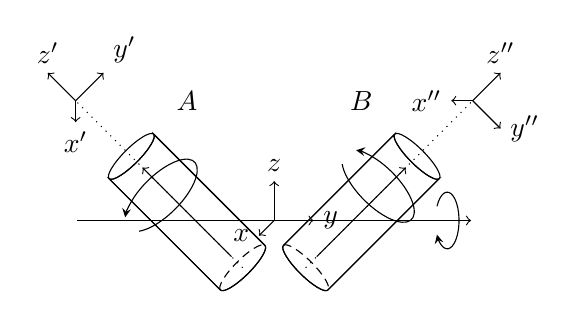
\begin{tikzpicture}[scale=1, transform shape]
    \begin{scope}[shift={(-0.4,0.0)}, rotate=45]
      \node[rotate=-45] at (1.0, 2.0) {$A$};

      \draw (0.4,0) -- (0.4,2.0) arc (360:180:0.4cm and 0.1cm) -- (-0.4,0) arc
      (180:360:0.4cm and 0.1cm);
      \draw (-0.4,2.0) -- (-0.4,0) arc (180:360:0.4cm and 0.1cm) -- (0.4,2.0) ++
      (-0.4,0) circle (0.4cm and 0.1cm);
      \draw[densely dashed] (-0.4,0) arc (180:0:0.4cm and 0.1cm);
      \draw[->] (0,0.2) -- (0,1.8) node[below]{$\AxisRotator[x=0.60cm,y=0.25cm]$};
      \draw[dotted] (0,0)--(0,3);
      \draw[->](0.0,3.0,0.0) -- (0.5, 3.0,0.0) node[above right,rotate=-45]{$y'$};
      \draw[->](0.0,3.0,0.) -- (0.0, 3.5,0.0) node[above,rotate=-45]{$z'$};
      \draw[->](0.0,3.0,0.0) -- (0.0, 3.0,0.5) node[below,rotate=-45]{$x'$};
    \end{scope}
    \begin{scope}[shift={(0.4,0.0)}, rotate=-45]
      \node[rotate=45] at (-1.0, 2.0) {$B$};

      \draw (0.4,0) -- (0.4,2.0) arc (360:180:0.4cm and 0.1cm) -- (-0.4,0) arc
      (180:360:0.4cm and 0.1cm);
      \draw (-0.4,2.0) -- (-0.4,0) arc (180:360:0.4cm and 0.1cm) -- (0.4,2.0) ++
      (-0.4,0) circle (0.4cm and 0.1cm);
      \draw[densely dashed] (-0.4,0) arc (180:0:0.4cm and 0.1cm);
      \draw[->] (0,0.2) -- (0,1.8) node[below]{$\AxisRotator[x=0.60cm,y=0.25cm]$};
      \draw[dotted] (0,0)--(0,3);
      \draw[->](0.0,3.0,0.0) -- (0.5, 3.0,0.0) node[right,rotate=45]{$y''$};
      \draw[->](0.0,3.0,0.) -- (0.0, 3.5,0.0) node[above,rotate=45]{$z''$};
      \draw[->](0.0,3.0,0.0) -- (0.0, 3.0,0.5) node[left,rotate=45]{$x''$};
    \end{scope}
    \draw[->] (-2.5,0.6)--(2.5,0.6) node[left]
    {$\AxisRotatorUnder[x=0.15cm,y=0.36cm]$};
    \draw[->](0.0,0.6,0.0) -- (0.5, 0.6,0.0) node[right]{$y$};
    \draw[->](0.0,0.6,0.) -- (0.0, 1.1,0.0) node[above]{$z$};
    \draw[->](0.0,0.6,0.0) -- (0.0, 0.6,0.5) node[left]{$x$};
  \end{tikzpicture}
   \end{center}
\end{figure}
\end{document}

  \caption{??? PLACE THIS SOMEWHERE}%
  \label{fig:cat_axis}
\end{figure}

\begin{figure}[htpb]
  \centering
  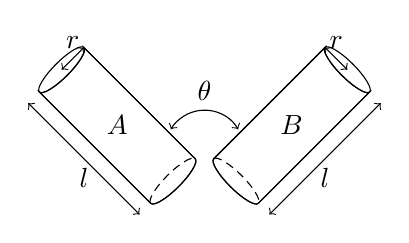
\begin{tikzpicture}[scale=1, transform shape]
  \begin{scope}[shift={(-0.4,0.0)}, rotate=45]
    \draw (0.4,0) -- (0.4,2.0) arc (360:180:0.4cm and 0.1cm) -- (-0.4,0) arc
    (180:360:0.4cm and 0.1cm);
    \draw (-0.4,2.0) -- (-0.4,0) arc (180:360:0.4cm and 0.1cm) -- (0.4,2.0) ++
    (-0.4,0) circle (0.4cm and 0.1cm);
    \draw[densely dashed] (-0.4,0) arc (180:0:0.4cm and 0.1cm);

    \draw[<->] (-0.6,0.0) -- node[below,midway,rotate=-45] {$l$} (-0.6, 2.0);
    \draw[<->] (0.0,2.0) -- node[above,midway,rotate=-45] {$r$} (0.4,2.0);

    \node[rotate=-45] at (0.0, 1.0) {$A$};
  \end{scope}
  \begin{scope}[shift={(0.4,0.0)}, rotate=-45]
    \draw (0.4,0) -- (0.4,2.0) arc (360:180:0.4cm and 0.1cm) -- (-0.4,0) arc
    (180:360:0.4cm and 0.1cm);
    \draw (-0.4,2.0) -- (-0.4,0) arc (180:360:0.4cm and 0.1cm) -- (0.4,2.0) ++
    (-0.4,0) circle (0.4cm and 0.1cm);
    \draw[densely dashed] (-0.4,0) arc (180:0:0.4cm and 0.1cm);

    \draw[<->] (0.6,0.0) -- node[below,midway,rotate=45] {$l$} (0.6, 2.0);
    \draw[<->] (-0.0,2.0) -- node[above,midway,rotate=45] {$r$} (-0.4,2.0);

    \node[rotate=45] at (0.0, 1.0) {$B$};
  \end{scope}
  \coordinate (A) at (-1,1);
  \coordinate (B) at (1,1);
  \coordinate (O) at (0,0.4);
  \pic[draw, <->, "$\theta$",angle eccentricity=1.5]{angle=B--O--A};
\end{tikzpicture}

  \caption{??? PLACE THIS SOMEWHERE}%
  \label{fig:cat_model}
\end{figure}

\section{Moment of Inertia of the Cat}
We model a falling cat with two cylinders $A$ and $B$ connected by a spherical joint (which we assume to be massless) with $A$ and $B$ separated by angle $\theta$.

\begin{claim}
  About the center of mass, the $y$ axis of the cat is principle. Further, we can write $\vec{L} = (2I_{yy})\omega_y\hat{y}$. For an $I_{yy}$ dependent on the geometry of the cylinders and $\theta$.
\end{claim}
\begin{proof}
  Let the moment of inertia tensors of cylinders $A$ and $B$ about the center of mass of the cat as a whole be denoted $I_A$ and $I_B$. Recall the definition of the moment of inertia tensor:
  \begin{equation*}
    I =
    \begin{pmatrix}
      \sum(y^2+z^2) & \sum xy       & \sum xz     \\
      \sum yx      & \sum(x^2+z^2) & \sum yz      \\
      \sum zx      & \sum zy       & \sum(x^2+y^2)
    \end{pmatrix}
  \end{equation*}
  Then, by the reflectional symmetry of bodies $A$ and $B$, the calculations for $I_A$ and $I_B$ are identical except for the replacement of $y$ by $-y$. So, we can safely write
  \begin{equation*}
    I_A =
    \begin{pmatrix}
      I_{xx} & I_{xy} & I_{xz} \\
      I_{yx} & I_{yy} & I_{yz} \\
      I_{zx} & I_{zy} & I_{zz}
    \end{pmatrix} \text{ and }
    I_B =
    \begin{pmatrix}
      I_{xx} & -I_{xy} & I_{xz} \\
      -I_{yx} & I_{yy} & -I_{yz} \\
      I_{zx} & -I_{zy} & I_{zz}
    \end{pmatrix},
  \end{equation*}
  And so the moment of inertia tensor $I$ of the cat as a whole is of the form
  \begin{equation*}
    I = I_A + I_B =
    \begin{pmatrix}
      2I_{xx} & 0       & 2I_{xz} \\
      0       & 2I_{yy} & 0 \\
      2I_{zx} & 0       & 2I_{zz}
    \end{pmatrix}
  \end{equation*}
  Then $\vec{y}$ is a clear eigenvector of $I$ confirming that the $y$ axis is a principle axis.
  \label{claim:principle}
\end{proof}
Note that the above argument can be generalized to any two bodies with reflectional symmetry through the $x,y$ plane.
\begin{claim}
  The $I_{yy}$ in claim \ref{claim:principle} can be written $I_{y'y'} \cos^2(\theta/2) + I_{z'z'} \sin^2(\theta/2)$ where $I_{y'y'}$ and $I_{z'z'}$ are the moment of inertia elements corresponding to the principle axes.
\end{claim}
\begin{proof}
  Let $x',y',z'$ denote the principle axes of cylinder $A$ about the center of mass with $z'$ going down the length of the cylinder, $x'$ parallel to $x$, and $y'$ in the corresponding location for a right-handed orthogonal coordinate system. Then, with this coordinate system corresponding to the principle axes, we can write the moment of inertia tenor $I_A'$ of cylinder $A$ about the center of mass of $A$.
  \begin{equation*}
    I_A =
    \begin{pmatrix}
      I_{x'x'} & 0 & 0 \\
      0 & I_{y'y'} & 0 \\
      0 & 0 & I_{z'z'}
    \end{pmatrix}
  \end{equation*}
  Now, we adjust to the $x,y,z$ coordinate system established above and solve for $I_{yy}$. Note $\hat{y}$ is given by $(0, \cos(\theta/2), \sin(\theta/2))$ in $x',y',z'$ coordinates. Thus by adjusting coordinates we have
  \begin{align*}
    I_{yy} &=
    \begin{pmatrix}
      0 & \cos(\theta/2) & \sin(\theta/2)
    \end{pmatrix}
    \begin{pmatrix}
      I_{x'x'} & 0 & 0 \\
      0 & I_{y'y'} & 0 \\
      0 & 0 & I_{z'z'}
    \end{pmatrix}
    \begin{pmatrix}
      0 \\ \cos(\theta/2) \\ \sin(\theta/2)
    \end{pmatrix}\\
    &= I_{y'y'} \cos^2(\theta/2) + I_{z'z'} \sin^2(\theta/2)
  \end{align*}
  The above gives the value of $I_{yy}$ about the center of mass of $A$, but the center of mass of the cat as a whole shares identical $x$ and $z$ values. So, by $I_{yy} = \sum x^2+z^2$, the value of $I_{yy}$ holds about the center of mass the cat.

\end{proof}
Again, note the above argument is generalizable given the principle axes.

Then overall we have a simple relationship between the angular momentum of the cat and an angular velocity $\omega$ of the cat in the $\vec{y}$ direction.

\begin{equation}
  \vec{L} = (I_{y'y'} \cos^2(\theta/2) + I_{z'z'} \sin^2(\theta/2))\omega \hat{y}
\end{equation}
In particular, if $A$ and $B$ are two solid cylinders of equal density with length $L$ and radius $R$, we have

\begin{equation}
  \vec{L} = (/**/)
\end{equation}

\section{????}

\section{Numerical Example}%
\label{sec:numerical_example}

\begin{figure}[htpb]
  \centering
  \begin{tikzpicture}[scale=1, transform shape]
  \begin{scope}[shift={(-0.4,0.0)}, rotate=45]
    \draw (0.4,0) -- (0.4,2.0) arc (360:180:0.4cm and 0.1cm) -- (-0.4,0) arc
    (180:360:0.4cm and 0.1cm);
    \draw (-0.4,2.0) -- (-0.4,0) arc (180:360:0.4cm and 0.1cm) -- (0.4,2.0) ++
    (-0.4,0) circle (0.4cm and 0.1cm);
    \draw[densely dashed] (-0.4,0) arc (180:0:0.4cm and 0.1cm);

    \draw[<->] (-0.6,0.0) -- node[below,midpoint,rotate=-45] {$1$} (-0.6, 2.0);
    \draw[<->] (0.0,2.0) -- node[above left,midpoint,rotate=-45] {$0.1$} (0.4,2.0);

    \node[rotate=-45] at (0.0, 1.0) {$A$};
  \end{scope}
  \begin{scope}[shift={(0.4,0.0)}, rotate=-45]
    \draw (0.4,0) -- (0.4,2.0) arc (360:180:0.4cm and 0.1cm) -- (-0.4,0) arc
    (180:360:0.4cm and 0.1cm);
    \draw (-0.4,2.0) -- (-0.4,0) arc (180:360:0.4cm and 0.1cm) -- (0.4,2.0) ++
    (-0.4,0) circle (0.4cm and 0.1cm);
    \draw[densely dashed] (-0.4,0) arc (180:0:0.4cm and 0.1cm);

    \draw[<->] (0.6,0.0) -- node[below,midpoint,rotate=45] {$1$} (0.6, 2.0);
    \draw[<->] (-0.0,2.0) -- node[above right,midpoint,rotate=45] {$0.1$} (-0.4,2.0);

    \node[rotate=45] at (0.0, 1.0) {$B$};
  \end{scope}
  \coordinate (A) at (-1,1);
  \coordinate (B) at (1,1);
  \coordinate (O) at (0,0.4);
  \pic[draw, <->, "$\frac{\pi}{4}$",angle eccentricity=1.5]{angle=B--O--A};
\end{tikzpicture}

  \caption{Specific model of cat for example}%
  \label{fig:example_cat}
\end{figure}

Here we will consider a physical example using our model of a cat, to compute
all of the necessary values. We will consider a cat of $\mathtt{mass}=m=1$,
$\mathtt{length}=l=1$, radius $\mathtt{radius}=r=0.1$, and maximum angle of
bend $\theta=\frac{\pi}{4}$. We will also consider the cat to be dropped from a
height of $10$, and with standard gravity of $-9.8$. The model of this cat is
depicted in Figure \ref{fig:example_cat}.

The first step is to compute the time that the cat has to do the rotation. We
find this simply using basic kinematics
\begin{align*}
  \Delta t = \sqrt{\frac{2h}{g}}=\sqrt{\frac{2\cdot 10}{9.8}}\approx 1.428.
\end{align*}

Next we will also compute the moment of inertia $I$, and to compute this
we require the inertia tensor for each of the cylinders individually. So we
compute these to be
\begin{align*}
   \begin{pmatrix}
     \frac{m}{12}\left(r^2+l^2\right) & 0 & 0\\
     0 & \frac{m}{12}\left(r^2+l^2\right) & 0\\
     0 & 0 & \frac{mr^2}{2}
   \end{pmatrix}\approx
   \begin{pmatrix}
     0.084 & 0 & 0\\
     0 & 0.084 & 0\\
     0 & 0 & 0.005
   \end{pmatrix}.
\end{align*}
Since both $A$ and $B$ cylinders are identical, then this is the inertia tensor
for both of them. The next stage is to compute the moment of inertia in the
$\vec{y}$ axis.
\begin{align*}
   I_{yy}=I_{y'y'}\cos^2\left(\frac{\theta}{2}\right)+I_{z'z'}\sin^2\left(\frac{\theta}{2}\right)\approx0.071841+0.000732\approx0.0726.
\end{align*}
Then from our previous computation, we evaluate for the rotational speed of the
cylinders $\omega$. We compute this as
\begin{align*}
  \omega=\frac{\pi}{\Delta
    t\left(1-\frac{I_{z'z'}}{I_{yy}}\sin\left(\frac{\theta}{2}\right)\right)}\approx2.2514.
\end{align*}
This is the rate that each cylinder must rotate at in order for the full
rotation to occurs.

To verify that this rate will work, we compute
\begin{align*}
  \int_0^{\Delta
    t}&\omega\left(1-\frac{I_{z'z'}}{I_{yy}}\sin\left(\frac{\theta}{2}\right)\right)dt\\
  &=\frac{\pi}{\Delta t}\int_{0}^{\Delta t}dt=\pi.
\end{align*}
Now we can compute the maximum amount of torque that the cat would require to
preform the rotation motion. This is given by
\begin{align*}
  \max(\tau_2)=\omega\frac{\pi}{\Delta t}I_*.
\end{align*}
We compute $I_*$ by the use of the parallel axis theorem. So we find
\begin{align*}
   I_*=I_{x'x'}+md=\frac{m}{12}\left(r^2+l^2\right)+m\frac{h^2}{4}=\frac{m}{12}\left(r^2+4l^2\right)\approx=0.3342.
\end{align*}
This is the moment of rotation of the cylinder about its end. Now we can use
this to compute the maximum torque required.
\begin{align*}
  \max(\tau_2)=\omega\frac{\pi}{\Delta t}I_*=\frac{\pi^2I_*}{\Delta
    t^2\left(1-\frac{I_{z'z'}}{I_{yy}}\sin\left(\frac{\theta}{2}\right)\right)}\approx1.655N.
\end{align*}

\section{Simulation}%
\label{sec:simulation}

To verify our computations, we constructed a software simulation, that would be
easily configurable, to allow rapid development. For the simulation we chose to
use the \texttt{Python} programming language, and to make use of the
\texttt{pyBullet} physics simulator. \texttt{pyBullet} is provided using
python's integrated package manager \texttt{pip}.

\subsection{URDF File Format}%
\label{sub:urdf_file_format}

\texttt{pyBullet} makes use of the \texttt{URDF} file format, so all models in
the simulation must be loaded from a urdf file. This format has some specific
constraints that are explained here, and the cat model that we used is
included. The urdf file type is a subset of XML.

The model is constructed with \texttt{links} and \texttt{joints}, and the
entire format is contained within a \texttt{robot} object.

\subsubsection{Link}%
\label{ssub:Link}

The link object can contains three sub objects, \texttt{visual}
\texttt{collision}, and \texttt{inertial}. The visual and collision objects,
can define a \texttt{geometry}, which can in turn be constructed from a few
selected primitives. And they can also define an \texttt{origin} object. The
geometry is used to determine the visual display, or the collision geometry
accordingly, and the origin object defines the orientation and the position of
the link relative to the robots origin.

The \texttt{inertial} object can define the components mass, and its inertial
tensor, along with the origin for the inertial computation. For most purposes
the origins for all three of these components can be the same, and the geometry
of the visual and collision components can also be the same.

\subsubsection{Joint}%
\label{ssub:joint}

The joint object defines the connections between the different links. Each
joint has a parent link and a child link, and an origin. The types of joints
that are available are a fixed joint, where no motion is permitted, a revolute
joint, which is rotation about a single axis, and a slide joint, which is an in
and out motion. Each of these different types of joints have different
parameters that need to be defined for each of them. Our model only makes use
of the fixed joints, and the revolute joints.

For the revolute joint, we must also define the axis for its rotation and the
limits of angles for the rotation.

\subsubsection{Construction}%
\label{ssub:construction}

To construct the cat with variable parameters, we wrote a script to generate
the \texttt{urdf} file altering the parameters to be what we desired.

\subsection{Simulation Setup}%
\label{sub:simulation_setup}

\texttt{pyBullet} provides all of the physics simulations that are necessary
for most common applications, but first it must be initialized in the code. To
do this one must use the following commands before any physics simulation is
possible.
\begin{minted}{python}
  import pybullet as p
  physicsClient = p.connect(p.GUI)
  p.setAdditionalSearchPath(pybullet_data.getDataPath())
\end{minted}
These commands initialize the graphical interface for the simulation, and
includes a path for some standard \texttt{pyBullet} models.

The next step is to set global constants that are persistent for the entirety
of the simulation. In this case we will only set the gravitational constant.
\begin{minted}{python}
  p.setGravity(0,0,-9.8)
\end{minted}
This function sets the gravitational force in the $x$, $y$, and $z$ directions.

The final step before beginning the simulation is to load any models that will
be used in the simulation. For our purposes, we load the standard
\texttt{plane.urdf}, and we load our constructed \texttt{cat.urdf}.
\begin{minted}{python}
  planeId = p.loadURDF("plane.urdf")
  startPos = [0,0,10]
  startOrientation = p.getQuaternionFromEuler([0,0,0])
  catId = p.loadURDF("cat.urdf",startPos, startOrientation)
\end{minted}
These functions load the plane model positioned at the origin, and loads the
cat model positioned at $(0,0,10)$, with the default orientation.

\subsection{Simulation Computation}%
\label{sub:simulation_computation}

With our our organization of the simulation, we are able to compute all
necessary values prior to the execution of the simulation. This process is
implementing the equations that we found previously, and computing their
numerical values for the provided model of the cat. The first stage is
computing the time that the cat has to preform the maneuver, and partitioning
that time for the three different stages of the motion.
\begin{minted}{python}
  t_max = np.sqrt(2 * 10 / 9.8)
  step_2 = 2 * t_max / 10
  step_3 = 8 * t_max / 10
  dt = (step_3 - step_2)
\end{minted}
Next we compute the moment of inertia.
\begin{minted}{python}
  ix = 1/12 * mass * (radius**2 + length**2)
  iy = 1/12 * mass * (radius**2 + length**2)
  iy = 1/2 * mass * radius**2
  ic = iy * np.cos(theta / 2.0)**2 + iz * np.sin(theta / 2.0)**2
  c = 1 - 2 * iz / (2 * ic) * np.sin(theta / 2.0)
\end{minted}
These first lines are computing the moment of inertia in the three principal
axes for each individual cylinder of the cat model. Next we compute the
combined moment of inertia, and a constant that we call $c$. This constant $c$
we derived previously. Now using the moment of inertia, and the time available
for the cat, we compute the rate at which the cat should rotate. Since this
will be variable with respect to time, we also construct a function to return
the rate of rotation.
\begin{minted}{python}
  omega_0 = np.pi / (dt * cloud)
  omega = lambda t: omega_0 * (-np.cos(np.pi / dt * t) + 1)
\end{minted}

\subsection{Simulation Execution}%
\label{sub:simulation_execution}

Now with all the components of the simulation constructed, we are able to run
the simulation. The entire code is presented below, and we will explain the
three stages of execution afterwards.

\begin{minted}{python}
while i < 1000:
  p.stepSimulation()
  if t < step_2:
    p.setJointMotorControlArray(catId, [0,2], p.POSITION_CONTROL,
    targetPositions=[(np.pi - theta) / 2.0 * (1 - np.cos(np.pi / step_2 *
    (t - step_2))),0])
  elif t < step_3:
    p.setJointMotorControlArray(catId, [0,2], p.POSITION_CONTROL,
    targetPositions[(np.pi - theta) * np.cos(phi), (np.pi - theta) * np.sin(phi)])
    phi += omega(t - step_2) / fps
  elif t < t_max:
    p.setJointMotorControlArray(catId, [0,2], p.POSITION_CONTROL,
    targetPositions=[x/2 * (1 + np.cos(np.pi / dt_3 * (t - step_3))), y/2 * (1
    + np.cos(np.pi / dt_3 * (t - step_3)))])
  t += 1.0 / fps
  i += 1
\end{minted}
The simulation can be broken into three steps. The first is the process of
bending the straight cat into the partially bent position. Then the next stage
is the rotational motion, which results in the reorientation. Then the final
stage is the straightening of the cat.



\end{document}
